\chapter{Power Delivery and Equivalent Circuits}
\label{chap:powerSuppliesDelivery}
Remember that one of the main purposes of electric circuits is to deliver power to devices. Often, we call these devices \textbf{loads}, because they load down a circuit by drawing power from that circuit. In order to maximize the amount of power that is delivered to a load from a particular circuit, we need to use some math to determine what the resistance of that load should be. Or, if the resistance (or impedance) of the device we are interested in powering is known, we need to design its driving circuitry according to that known load resistance (or impedance). Either way, the material covered in this chapter will facilitate those design decisions.
\par
\section{Driving Circuit for a Load}
In this chapter, I will refer to \textbf{driving circuits} for loads. By this, I mean everything in a circuit \textit{besides} the load in question. Consider Figure \ref{maxPowerLoadMatching}. This figure shows a simple driving circuit (encircled in the figure by a gray box) that powers a load. The internal voltage source for the driving circuit is denoted as $V_s$, the internal resistance for the driving circuit is represented as $R_s$, and the load resistance is represented as $R_L$. Any driving circuit that is designed to power a device can be represented by an \textbf{equivalent circuit}, which is comprised of an \textit{equivalent} internal source and an \textit{equivalent} internal resistance. When connected to such an equivalent circuit, the load in question will be powered identically by either the original driving circuit or its equivalent. We will learn ways to use this representation to simplify large circuits later in this chapter.
\begin{figure}[h!]
\centering
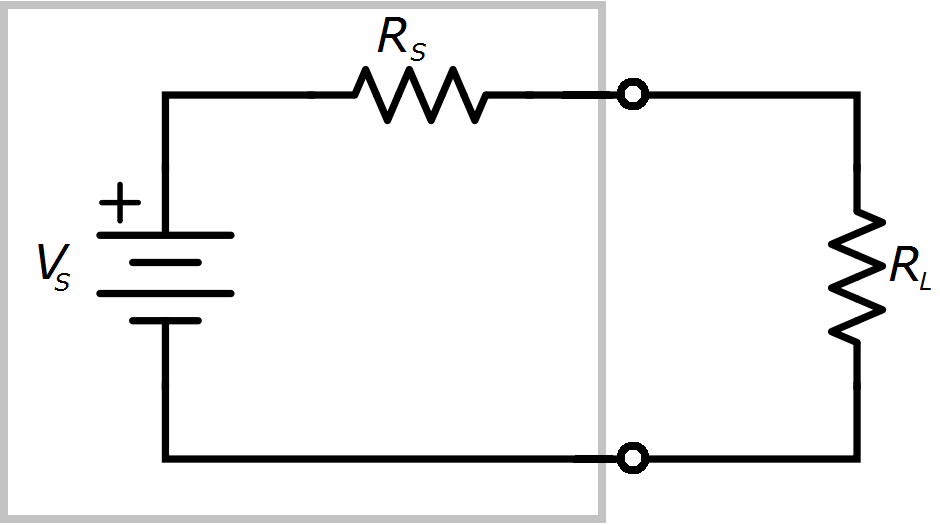
\includegraphics[width=13cm]{figures/maxPLoadMatching.png}
\caption{The simplest circuit for powering a load.}
\label{maxPowerLoadMatching}
\end{figure}
\par
The defining values for \textit{all} of the elements in the circuit of Figure \ref{maxPowerLoadMatching}---the internal voltage, internal resistance, \textit{and} the load resistance---will determine how much power is delivered to the load resistor. If the voltage is increased, it is clear that the power delivered to the load would also increase. However, assuming the voltage source is constant, what we really want to determine is how much power can be delivered to $R_L$ given the value of $R_s$.
\section{The Maximum Power Transfer Theorem}
Let's start our investigation using the voltage divider rule. $R_s$ and $R_L$ comprise a voltage divider, with $V_s$ applied across them both in series. The voltage across $R_L$ (which I will call $V_L$) is determined in the following way:
$$
V_L = V_s \cdot \left(\frac{R_L}{R_L + R_s}\right)
$$
Regardless of the values for $R_L$ and $R_s$, this expression is accurate. What we are most interested in is the power dissipated by $R_L$, and we can use one of the forms of Watt's Law in combination with this definition for $V_L$ to express the power provided to the load as 
$$
P_L = \frac{V_L^2}{R_L} = V_s^2 \cdot \left(\frac{R_L^{\bcancel{2}}}{(R_L + R_s)^2 \cdot \bcancel{R_L}}\right) = V_s^2 \cdot \left(\frac{R_L}{(R_L + R_s)^2}\right)
$$
\par
Now that we have an expression for power delivered to the load in terms of the internal circuit resistance $R_s$ and the load resistance $R_L$, we need to determine what configuration of these resistances will maximize the expression. This is an area where derivatives will come in handy! The derivative of the expression for $P_L$ with respect to $R_L$ is the slope of the function as we vary the value of $R_L$.
\begin{figure}[h!]
\centering
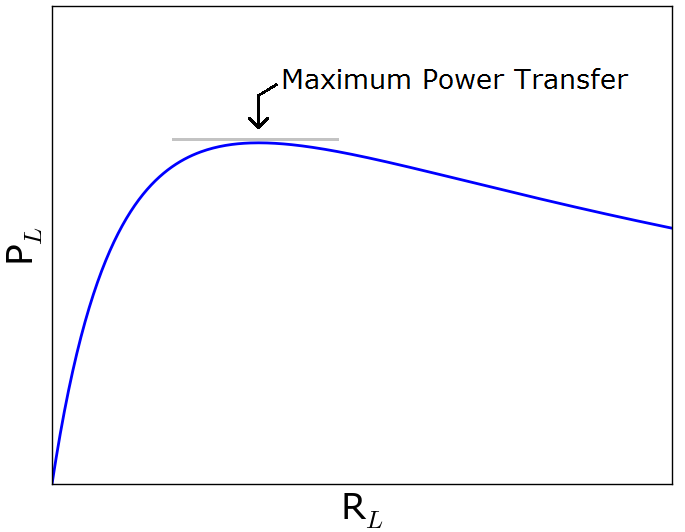
\includegraphics[width=13cm]{figures/PLvsRLrev1.png}
\caption{The shape of $P_L$ as a function of $R_L$. Maximum power is transferred to the load at the marked peak of the function.}
\label{PLvsRL}
\end{figure}
A sketch of the shape of $P_L(R_L)$ is shown in Figure \ref{PLvsRL}, and from it we can clearly see that there is a peak value. The function therefore has a derivative that passes through zero, and the specific argument used in the derivative that yields a result of zero will give the maximum value for the function itself. We're going to use that logic to find the \textit{value} for $R_L$ that maximizes power delivered \textit{to} $R_L$. 
\par
Concisely, we're going to 
\begin{enumerate}
\item{Take the derivative of $P_L$ with respect to $R_L$}
\item{Set the derivative equal to zero}
\item{Solve that equation for the value of $R_L$}
\end{enumerate}
So, taking the derivative of $P_L$ with respect to $R_L$ yields
$$
\frac{\mathrm{d}{P_L}}{\mathrm{d}R_L} = V_s^2 \cdot \frac{R_s^2-R_L^2}{(R_L + R_s)^4}
$$
\par
If we require that derivative to be zero and solve for the value of $R_L$ in that case, we find that $R_L=R_s$. This is the crux of the \textbf{Maximum Power Transfer Theorem}, which states that the maximum possible power will be transferred by the circuit to the load if the resistance of that load is equal to the internal resistance of the driving circuit. A major implication of this is that only half of the power dissipated by a circuit (at most!) can be transferred to a load.

\section{Thevenin and Norton Equivalent Circuits}
The behavior of any circuit that drives a specific load resistance ($R_L$) can be fully described by the current it causes to flow through the load and by the voltage it presents across that load. Any two circuits that provide the same current and voltage conditions to a load resistance can be described as \textbf{equivalent circuits}. Consider Figure \ref{blackboxDrivingCircuit}. The diagram on the left shows a load resistor being powered by an unknown driving circuit. For the purposes of determining power consumption by the load, the only circuit characteristics that matter are the current flowing through the load resistor and the voltage across that load. The circuits on the right of Figure \ref{blackboxDrivingCircuit} are each comprised of just two elements, but when the values of those elements are set appropriately, either of those circuits can produce the behavior of \textit{any} driving circuit for a load resistance. These two circuit types are named for their inventors---a voltage supply in series with a resistor is known as a \textbf{Thevenin equivalent circuit}, and a current supply in parallel with a resistor is known as a \textbf{Norton equivalent circuit}. 
\begin{figure}[h!]
\centering
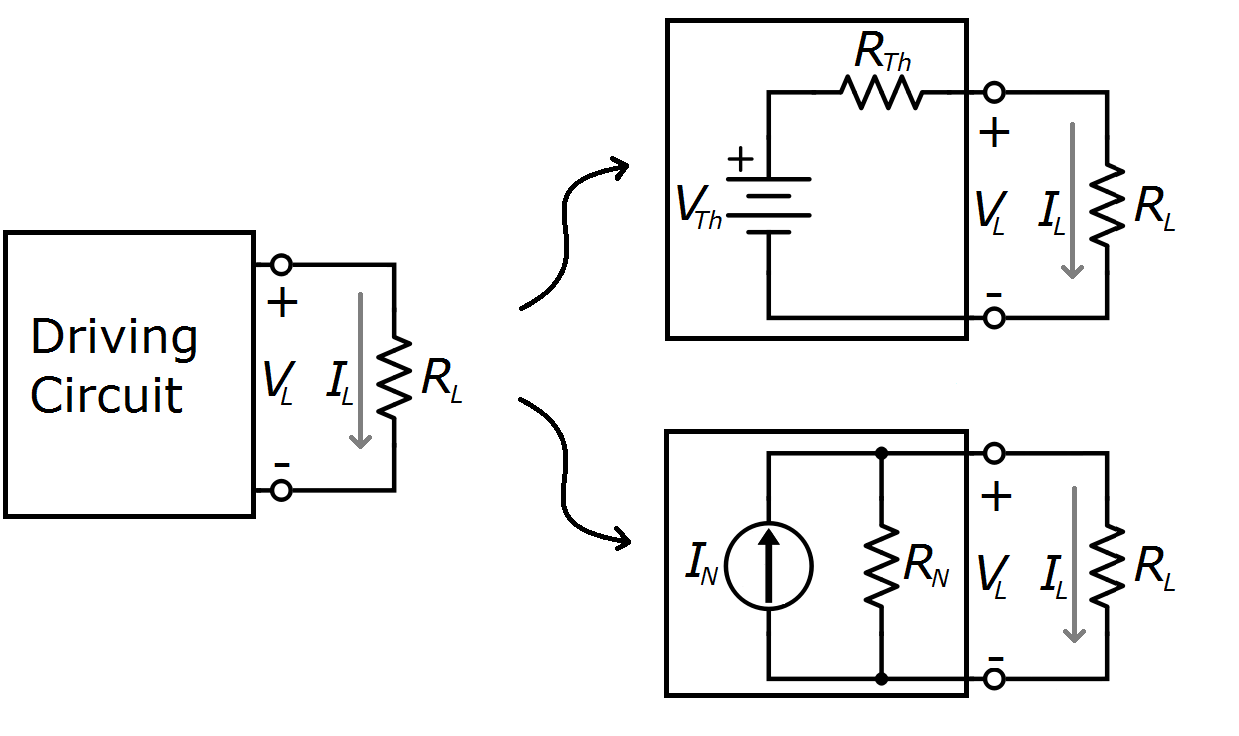
\includegraphics[width=13cm]{figures/blackboxDrivingToEquivalents.png}
\caption{The effect of a circuit on a load is described by the current flowing through that load and the voltage across the load. Regardless of the complexity of the actual driving circuit, the voltage and current characteristics of the driving circuit can be reproduced by either a voltage source in series with a resistor, or a current source in parallel with a resistor.}
\label{blackboxDrivingCircuit}
\end{figure}
\par
Like the resistor combination rules we learned in Chapter \ref{chap:resistorRulesAndTricks}, both of those equivalent circuit types can be used in the process of reducing larger circuits to smaller equivalent circuits. By recognizing that even in a larger circuit we can transform a voltage source in series with a resistor into a current source in parallel with a resistor and vice versa, we are empowered to perform these transformations while combining resistances in series and parallel to ultimately determine a single Norton or Thevenin equivalent circuit as ``seen'' by a load resistance in the larger circuit. Also, this process of transformation is quite simple. 
\par
To transform a Thevenin equivalent circuit into its corresponding Norton equivalent circuit, we need to determine how the Thevenin voltage and Thevenin resistance are related to the Norton current and Norton resistance. These releationships can be deduced from two quantities---the voltage across the two terminals where the element was connected to the circuit, and the current that would flow through a wire connecting those two terminals. These quantities are often referred to as the open-circuit voltage ($V_{oc}$) and the short-circuit current ($i_{sc}$), which are both represented in Figure \ref{ThevToNortFromOC_SC}. 
\begin{figure}[h!]
\centering
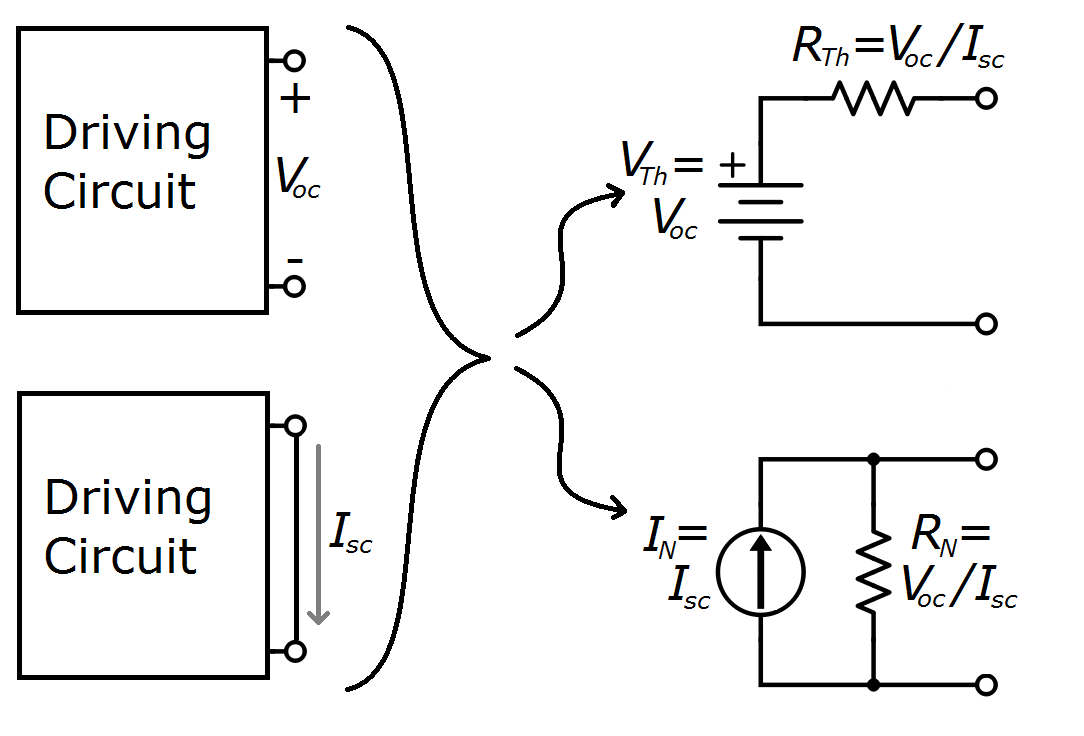
\includegraphics[width=10cm]{figures/thevNortFromOC_SC.png}
\caption{Given the open circuit voltage and closed circuit current between the two driving circuit terminals to which the load is connected, we can easily construct either a Thevenin or Norton equivalent circuit for the driving circuit. The equivalent resistance is the same for both the Thevenin and the Norton circuit.}
\label{ThevToNortFromOC_SC}
\end{figure}
With those quantities in hand, we can solve for the equivalent resistance and either the Thevenin equivalent voltage or the Norton equivalent current. The equivalent resistance is the same for either circuit:
$$
R_{Th} = R_{N} = \frac{V_{oc}}{i_{sc}}
$$
$$
V_{Th} = V_{oc}
$$
$$
i_{N} = i_{sc}
$$

These expressions confirm that converting from a Norton equivalent circuit to a Thevenin equivalent circuit and vice versa is easy. By doing so, we can simplify any resistive circuit that drives a load to its Norton or Thevenin equivalent by combining elements step by step.
\par
Let's put all this information to good use by determining the Thevenin and Norton equivalent circuits that the 1k$\Omega$ resistor in the circuit of Figure \ref{NortonTheveninEx1} ``sees'' by using the equivalent resistance combination tricks we learned in Chapter \ref{chap:resistorRulesAndTricks} in combination with the process of converting Thevenin circuits to Norton circuits and vice versa.
\begin{figure}[h!]
\centering
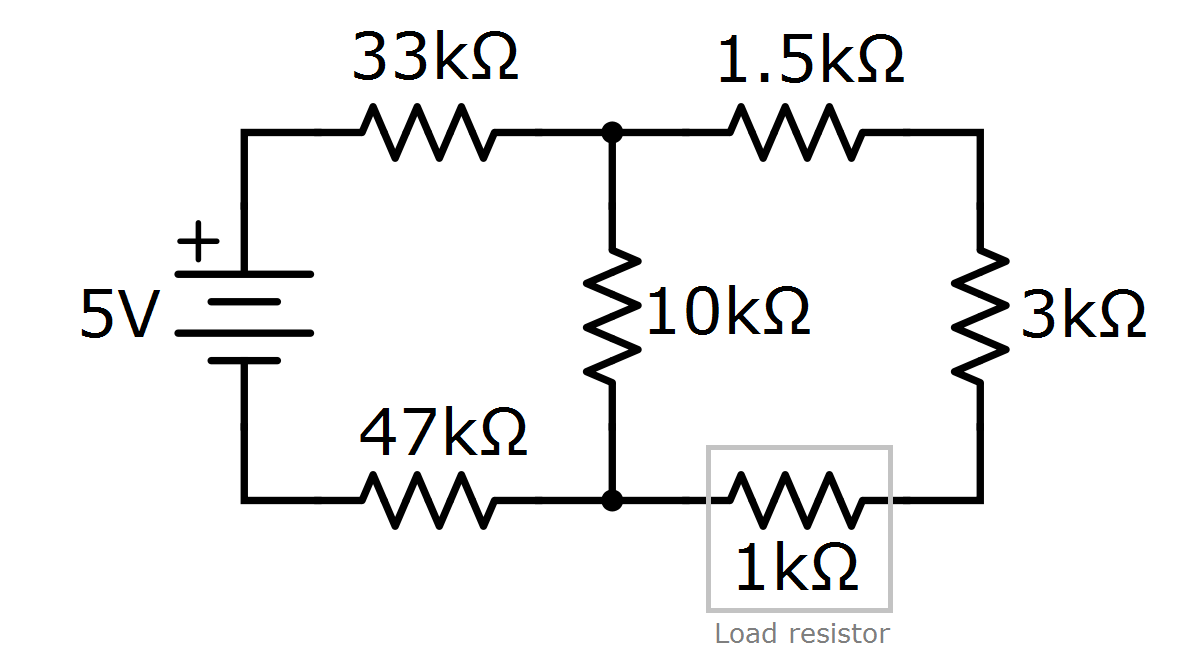
\includegraphics[width=15cm]{figures/nortThevEx_1.png}
\caption{A resistive circuit. For this example, we treat the 1k$\Omega$ resistor as the load.}
\label{NortonTheveninEx1}
\end{figure}
First, we want to take out the 1k$\Omega$ resistor, and leave open terminals at its position in the circuit. Then, we can begin simplifying the rest of the circuit that is connected to those terminals. In order to keep track of where those terminals are, it helps to redraw the remaining circuit before we continue, as shown in Figure \ref{NortonTheveninEx2}. Now, we are ready to simplify what is inside the gray box of this figure. 
\begin{figure}[h!]
\centering
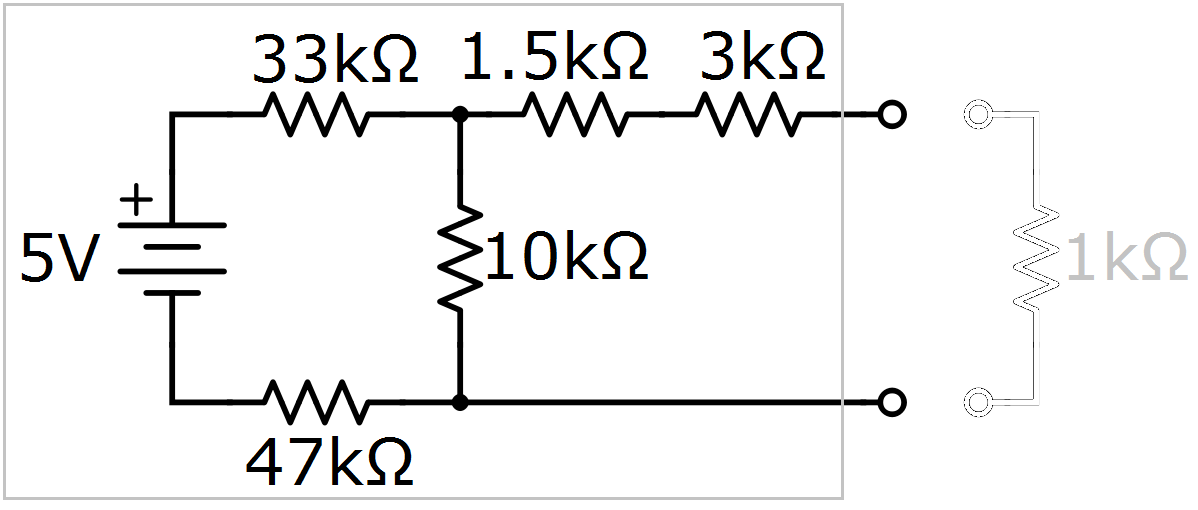
\includegraphics[width=15cm]{figures/nortThevEx_2.png}
\caption{With the 1k$\Omega$ load removed from the circuit, we simplify what is left while preserving the terminals for the load resistor.}
\label{NortonTheveninEx2}
\end{figure}
\par
Let's start by combining the 1.5k$\Omega$ and the 3k$\Omega$ resistors into an equivalent resistance of 4.5k$\Omega$ as shown in Figure \ref{NortonTheveninEx3}. At this point, there are no more obvious series or parallel resistors to combine, but if we look at the far left of the circuit, we see a 33k$\Omega$ resistor, a 47k$\Omega$ resistor, and a voltage source all in series. We can deduce that the Thevenin equivalent configuration of those three elements is a 5V source in series with a single 80k$\Omega$ resistor, as shown in Figure \ref{NortonTheveninEx4}.
\begin{figure}[h!]
\centering
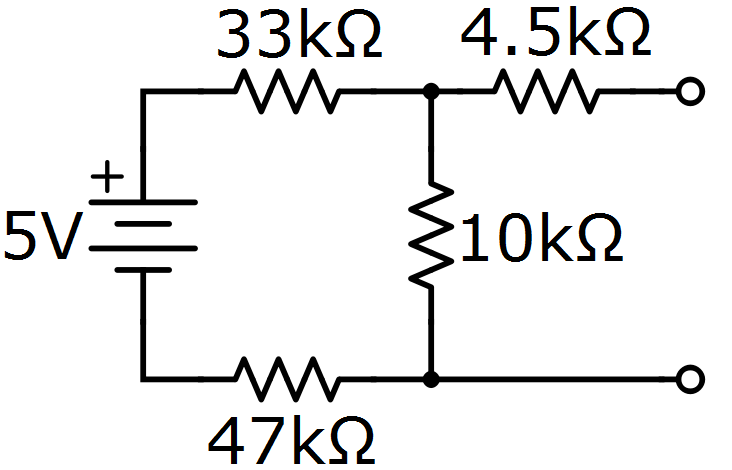
\includegraphics[width=10cm]{figures/nortThevEx_3.png}
\caption{The driving circuit after combining the series 1.5k$\Omega$ and 3k$\Omega$ resistors.}
\label{NortonTheveninEx3}
\end{figure}

\begin{figure}[h!]
\centering
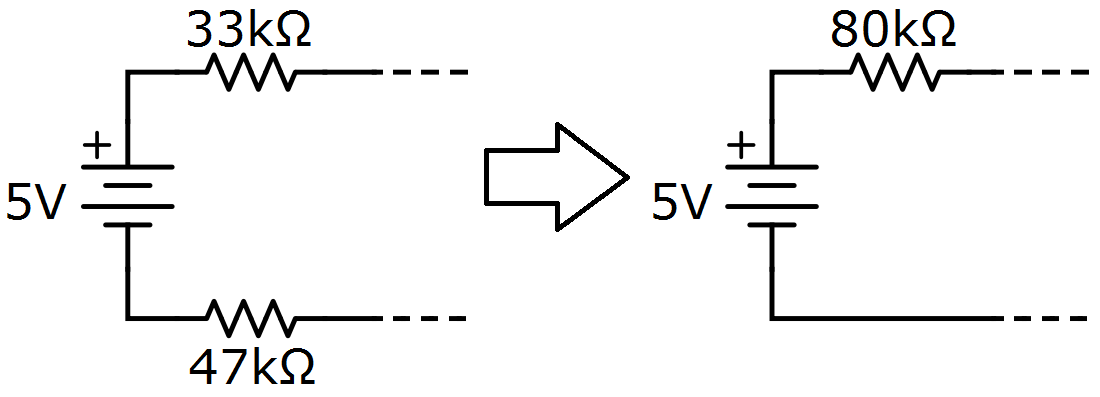
\includegraphics[width=15cm]{figures/nortThevEx_4.png}
\caption{The voltage source and two resistors at the far left of the circuit can be reconfigured as a Thevenin equivalent circuit as shown here.}
\label{NortonTheveninEx4}
\end{figure}
\par
Having found this Thevenin equivalent circuit, we can transform it into a Norton equivalent with a 62.5mA Norton current source (because 5V/80k$\Omega$=62.5mA) in parallel with an 80k$\Omega$ resistance. The resulting circuit is shown in Figure \ref{NortonTheveninEx5}. Note that now the 80k$\Omega$ and 10k$\Omega$ resistors are in parallel, and we can therefore combine them into a single 8.9k$\Omega$ resistance as shown in Figure \ref{NortonTheveninEx6}.
\begin{figure}[h!]
\centering
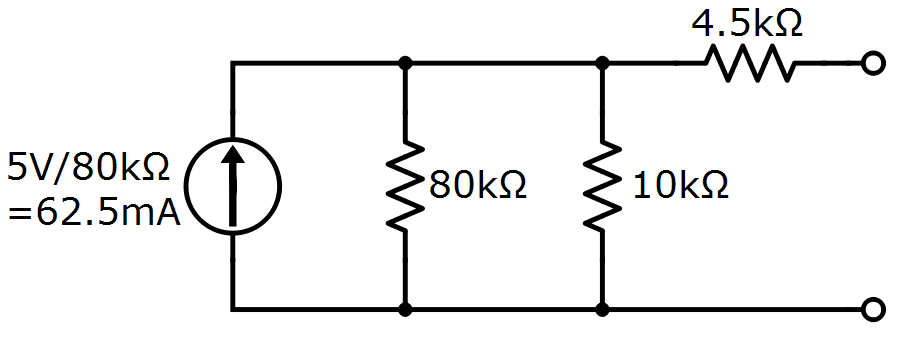
\includegraphics[width=15cm]{figures/nortThevEx_5.png}
\caption{After transforming the Thevenin equivalent circuit to a Norton equivalent, we see that the 80k$\Omega$ and 10k$\Omega$ resistors in the resulting circuit are in parallel.}
\label{NortonTheveninEx5}
\end{figure}

\begin{figure}[h!]
\centering
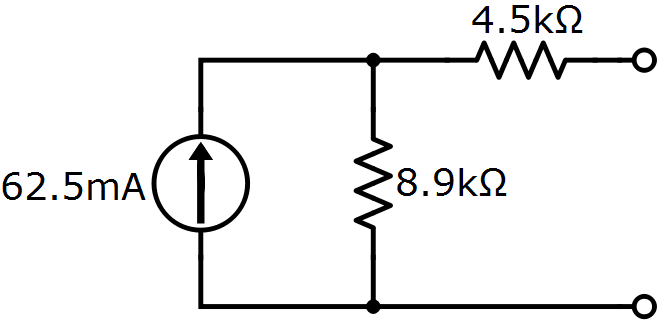
\includegraphics[width=10cm]{figures/nortThevEx_6.png}
\caption{The 80k$\Omega$ and 10k$\Omega$ resistors have been combined.}
\label{NortonTheveninEx6}
\end{figure}
\par
At this point, we've managed to pare our initial driving circuit down to just two resistors and one current source. Let's insert a Thevenin equivalent representation in place of the Norton circuit comprised of the 62.5mA current source and the 8.9k$\Omega$ resistor. That Thevenin equivalent has a voltage of 0.56V as shown in Figure \ref{NortonTheveninEx7}. The last simplification step to finding the Thevenin equivalent circuit as seen by the 1k$\Omega$ resistor is to replace the 8.9k$\Omega$ and 4.5k$\Omega$ resistors with a single 13.4k$\Omega$ resistor. The resulting Thevenin equivalent and Norton equivalent circuits are shown in Figure \ref{NortonTheveninEx8}.
\begin{figure}[h!]
\centering
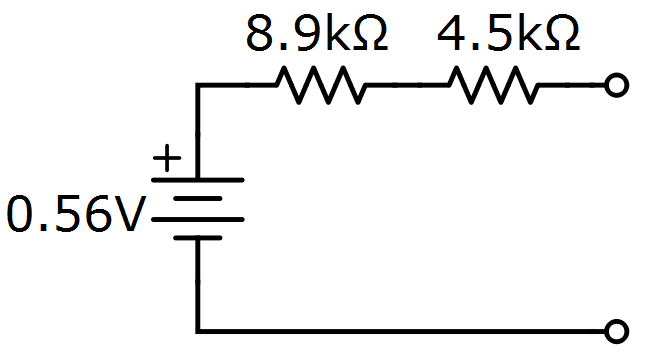
\includegraphics[width=10cm]{figures/nortThevEx_7.png}
\caption{The 62.5mA current source in parallel with the 8.9k$\Omega$ resistor (a Norton circuit) have been transformed into their Thevenin equivalent circuit.}
\label{NortonTheveninEx7}
\end{figure}

\begin{figure}[h!]
\centering
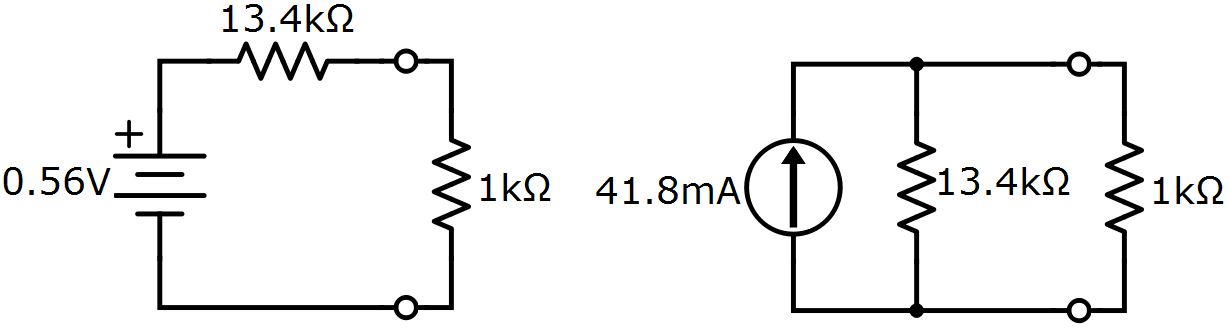
\includegraphics[width=15cm]{figures/nortThevEx_8.png}
\caption{After combining the 8.9k$\Omega$ and 4.5k$\Omega$ series resistors, the internal  resistance for the driving circuit has been found to be 13.4k$\Omega$. The Thevenin and Norton equivalent circuits as ``seen'' by the 1k$\Omega$ load resistance are shown here.}
\label{NortonTheveninEx8}
\end{figure}
\par
At this point, we can clearly see that this circuit does not deliver the maximum amount of power possible to the 1k$\Omega$ load, because the internal resistance of the circuit is 13.4k$\Omega$ rather than 1k$\Omega$. While the internal resistance of the initial circuit of Figure \ref{NortonTheveninEx1} was not obvious, reducing driving circuits to their Thevenin and Norton equivalent representations like we have done in this example makes it easy to determine what value of load resistance would maximize power delivery. 

\section{Recap: Maximum Power Transfer Theorem}
In this chapter, we learned that every circuit that drives a load resistance has an internal resistance. Even real power supplies have internal resistance. This internal resistance ties together the concepts we learned about in this chapter, namely
\begin{description}
\item[Load:] An element in a circuit for which that circuit was designed to provide power.
\item[Driving Circuit:] A circuit that is designed to power a load.
\item[Maximum Power Transfer Theorem:] The maximum possible power that a driving circuit can provide to a load will only be transferred by the circuit to the load if the resistance of that load is equal to the internal resistance of the driving circuit. Therefore, the efficiency of power delivery in electric circuits can be at most 50$\%$.
\item[Equivalent Circuits:] Equivalent circuits are circuits that provide the same voltage across and current through a load resistance. 
\item[Thevenin Equivalent Circuit:] A Thevenin equivalent circuit is comprised of just one voltage source in series with just one resistance. No matter how complicated the actual driving circuit, a Thevenin equivalent circuit can emulate the current and voltage conditions experienced by a load resistance. 
\item[Norton Equivalent Circuit:] A Norton equivalent circuit is comprised of just one current source in parallel with just one resistance. No matter how complicated the actual driving circuit, a Norton equivalent circuit can emulate the current and voltage conditions experienced by a load resistance. 
\end{description}
